\documentclass[a4paper,11pt]{article}
\usepackage{amsmath,amsthm,amsfonts,amssymb,amscd,amstext,vmargin,graphics,graphicx,tabularx,multicol} 
\usepackage[francais]{babel}
\usepackage[utf8]{inputenc}  
\usepackage[T1]{fontenc} 
\usepackage{pstricks-add,tikz,tkz-tab,variations}
\usepackage[autolanguage,np]{numprint} 


\setmarginsrb{2.5cm}{0.5cm}{2.5cm}{2cm}{0cm}{0cm}{0cm}{0cm} %Gauche, haut, droite, haut
\newcounter{numexo}
\newcommand{\exo}[1]{\stepcounter{numexo}\noindent{\bf Exercice~\thenumexo} : \marginpar{\hfill /#1}}
\reversemarginpar


\newcounter{enumtabi}
\newcounter{enumtaba}
\newcommand{\q}{\textbf{\stepcounter{enumtabi} \theenumtabi)}  }
\newcommand{\qa}{\textbf{\stepcounter{enumtaba} (\alph{enumtaba})} }
\newcommand{\initq}{\setcounter{enumtabi}{0}}
\newcommand{\initqa}{\setcounter{enumtaba}{0}}

\newcommand{\be}{\begin{enumerate}}
\newcommand{\ee}{\end{enumerate}}
\newcommand{\bi}{\begin{itemize}}
\newcommand{\ei}{\end{itemize}}
\newcommand{\bp}{\begin{pspicture*}}
\newcommand{\ep}{\end{pspicture*}}
\newcommand{\bt}{\begin{tabular}}
\newcommand{\et}{\end{tabular}}
\renewcommand{\tabularxcolumn}[1]{>{\centering}m{#1}} %(colonne m{} centrée, au lieu de p par défault) 
\newcommand{\tnl}{\tabularnewline}

\newcommand{\bmul}[1]{\begin{multicols}{#1}}
\newcommand{\emul}{\end{multicols}}

\newcommand{\trait}{\noindent \rule{\linewidth}{0.2mm}}
\newcommand{\hs}[1]{\hspace{#1}}
\newcommand{\vs}[1]{\vspace{#1}}

\newcommand{\N}{\mathbb{N}}
\newcommand{\Z}{\mathbb{Z}}
\newcommand{\R}{\mathbb{R}}
\newcommand{\C}{\mathbb{C}}
\newcommand{\Dcal}{\mathcal{D}}
\newcommand{\Ccal}{\mathcal{C}}
\newcommand{\mc}{\mathcal}

\newcommand{\vect}[1]{\overrightarrow{#1}}
\newcommand{\ds}{\displaystyle}
\newcommand{\eq}{\quad \Leftrightarrow \quad}
\newcommand{\vecti}{\vec{\imath}}
\newcommand{\vectj}{\vec{\jmath}}
\newcommand{\Oij}{(O;\vec{\imath}, \vec{\jmath})}
\newcommand{\OIJ}{(O;I,J)}


\newcommand{\reponse}[1][1]{%
\multido{}{#1}{\makebox[\linewidth]{\rule[0pt]{0pt}{20pt}\dotfill}
}}

\newcommand{\titre}[5] 
% #1: titre #2: haut gauche #3: bas gauche #4: haut droite #5: bas droite
{
\noindent #2 \hfill #4 \\
#3 \hfill #5

\vspace{-1.6cm}

\begin{center}\rule{6cm}{0.5mm}\end{center}
\vspace{0.2cm}
\begin{center}{\large{\textbf{#1}}}\end{center}
\begin{center}\rule{6cm}{0.5mm}\end{center}
}


\begin{document}
\pagestyle{empty}
\titre{Interrogation - Construction de vecteurs}{Nom :}{Prénom :}{\textbf{2nd}}{Sujet A}

\vspace*{0.25cm}
\exo{2} COURS \\
\initq \q Comment caractérise-t-on le vecteur $-\overrightarrow{u}$ par rapport au vecteur $\overrightarrow{u}$ ?\\
  \reponse[3]\\
  \q Donner la définition du vecteur nul ?\\
  \reponse[3]\\
  \q Compléter la propriété suivante :\\
  "$\overrightarrow{RF}=\overrightarrow{RD}$ si et seulement si . . . . . . . . . . . . . . . . . . . . . . . . . . . . . . . . . . . . . . . . . . ."\\
  
  \vspace*{0.5cm}
\exo{2} Dans chacun des cas de la figure suivante, construire en rouge le vecteur $\overrightarrow{w}$ d'origne A puis d'origine B tel que $\overrightarrow{w}=\overrightarrow{u}+\overrightarrow{v}$.\\
  \includegraphics[scale=1.5]{sommeinterro1.eps} \\
  
  
  
  
  \exo{2} Pour chacune des propositions suivantes, dire si elle est vrai ou fausse. Aucune justification n'est demandée.\\
  \initq \q Si F est l'image de A par la translation de vecteur $\overrightarrow{GT}$ alors $\overrightarrow{GT}=\overrightarrow{AF}$.\\
  \q Si $\overrightarrow{FE}=\overrightarrow{RU}$ alors FERU est un parallélogramme.\\
  \q Si $\overrightarrow{DE}=-\overrightarrow{EA}$ alors E est le milieu du segment [DA].\\
  \q Si K est le symétrique de T par rapport à L alors $\overrightarrow{KL}=\overrightarrow{LT}$\\
   \reponse[5]\\
  
  \newpage
  \vspace*{0.5cm}
  \exo{4} On considère l'hexagone ABCDEF ci-dessous.\\
  
  \includegraphics[scale=1.5]{exo2cours.eps} \\
  
 \noindent \initq \q Nommer le représentant du vecteur $\overrightarrow{EF}$ d'origine O.\\
  \q Citer deux vecteurs égaux au vecteur $-\overrightarrow{FA}$.\\
  \q Construire N l'image du point C tel que $\overrightarrow{CN}=\overrightarrow{OB}$.\\
  \q  Construire M l'image du point D tel que $\overrightarrow{DM}=2\overrightarrow{AB}$.\\
  \q Construire P l'image du point O tel que $\overrightarrow{OP}=\dfrac{1}{3}\overrightarrow{EM}-\overrightarrow{CB}$.\\
   \reponse[5]\\
  
\end{document}
